% !TEX root = ../main.tex
\section{Analýza pôvodného stavu robota}
\label{sec:formerState}

\subsection{Robot a~jeho ovládanie}
\label{subsec:robotAOvladanie}

Robot, s~ktorým sme pracovali bol výsledkom tímového projektu viacerých študentov \newline z~roku 2019. Pri~vysvetľovaní
a~opisovaní robota sa budeme odvolávať na~dokumenty, stránky a~kód, ktorý napísali. Všetky tieto údaje sú~sprístupnené
na~mobilnom robote v~záložke \newline \texttt{\$(HOME)/Desktop/Blackmetal}~\cite{timovyProjekt}.

Robot je v~tvare kvádra. Jeho šírka je 60cm a~je vyzdvihnutý nad zem o~1.5cm. Nachádza sa na~kolesách o~polomere 8cm.
Jeho kostra sa skladá z~dvoch oceľových plátov, ktoré tvoria dno a~strechu robota. Steny robota sú~spravené z~hliníku.
Konkrétne z~hliníkových tyčí, ktoré sú~pospájané plexisklovými plátmi. Jeho podobizeň vidíme na~nasledujúcom
obrázku.

\begin{figure}[!htbp]
	\begin{center}
		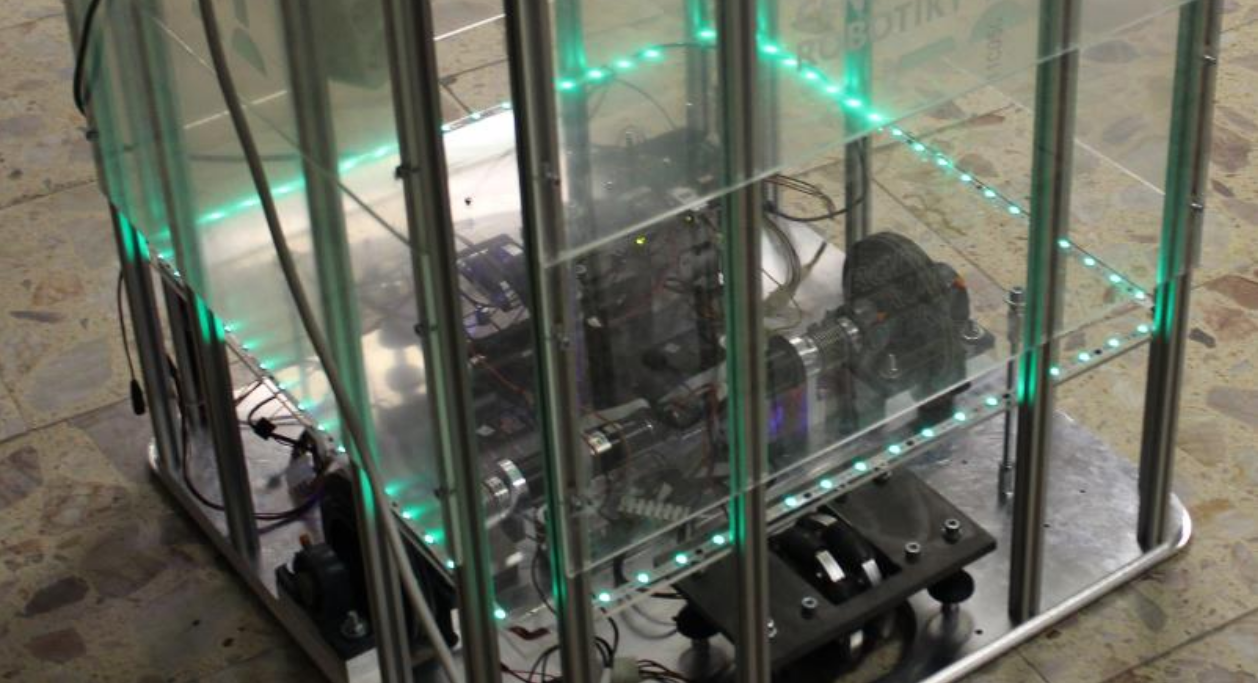
\includegraphics[width=0.95\textwidth]{img/robot.png}
	\end{center}
	\caption{Zobrazenie spodnej časti mobilného robota~\cite{timovyProjekt}}
	\label{fig:robot}
\end{figure}

Na~obrázku ďalej vidíme olemovanie robota pásom s~LED-kami. Tie svietia nasledovným spôsobom. Keď sa robot nehýbe
všetky LED-ky svietia na~zeleno. Keď sa robot pohne do~nejakej strany, LED-ky znázornia jeho pohyb tým, že~svietia
na~modro na~strane, do~ktorej sa robot hýbe a~na~červeno na~všetkých ostatných stranách. Keď nastane situácia,
kedy počítač ovládajúci motory prestane komunikovať s~Arduinom, ktoré sa stará o~detekciu stavov robota
tak~LED-ky začnú blikať červeno-modrými farbami.

\clearpage

Ako bolo spomenuté LED-ky znázorňujú pohyb robota. Ten sa pohybuje za~pomoci diferenciálneho podvozku s~dvoma
podpornými všesmerovými kolesami. Motory robota sú~pripojené na~meniče. Tie sú~ovládané priamo príkazmi z~počítača.\\

\noindent Hardware robota sa skladá z:
\begin{itemize}
	\item kontrolnej dosky Arduino Uno,

	\item Počítača ADVANTECH MIO-5272 \newline
		Počítač obsahuje operačný systém založený na~jadre Linux Ubuntu 16.04~\cite{robotPc}.

	\item Extension board MIOe-210~\cite{extensionModule}

	\item Meniče MAXON EPOS 24/5 (s~číslom 275512) \newline
	 	Meniče sú~napájané jednosmerným napätím 11 - 24 V~a~5 A~\cite{menic}.

	\item Enkódery MAXON Encoder MR Type L (s~číslom 225787) \newline
		Rozlíšenie enkóderov je 1024 impulzov s~troma kanálmi~\cite{encoder}.

	\item Motory MAXON RE 40 (s~číslom 148867) \newline
		Motory s~výkonom 150W. Maximálna rýchlosť je 12 000 rpm a~efektivita 91\%~\cite{motor}.

	\item Prevodovka MAXON Planetary Gearhead GP 42 C (s~číslom 202120) \newline
		Redukcia prevodovky je 43:1. Jej účinnosť je 72\%~\cite{prevodovka}.
\end{itemize}

\noindent Ovládanie robota je zabezpečené externými počítačmi
\begin{itemize}
	\item Control PC (Kontrolný počítač) -- Počítač posielajúci príkazy na~robot cez~TCP/IP protokol.
	\item Logging PC (Logovací počítač) -- Počítač prijímajúci stav robota cez~TCP/IP protokol.
\end{itemize}

\noindent Tieto počítače sú~len reprezentáciou dvoch klientov pripájajúcich sa na~dva separátne porty na~robote.
V~realite to~môže byť jeden a~ten istý počítač.

\clearpage

\begin{figure}[!htbp]
	\begin{center}
		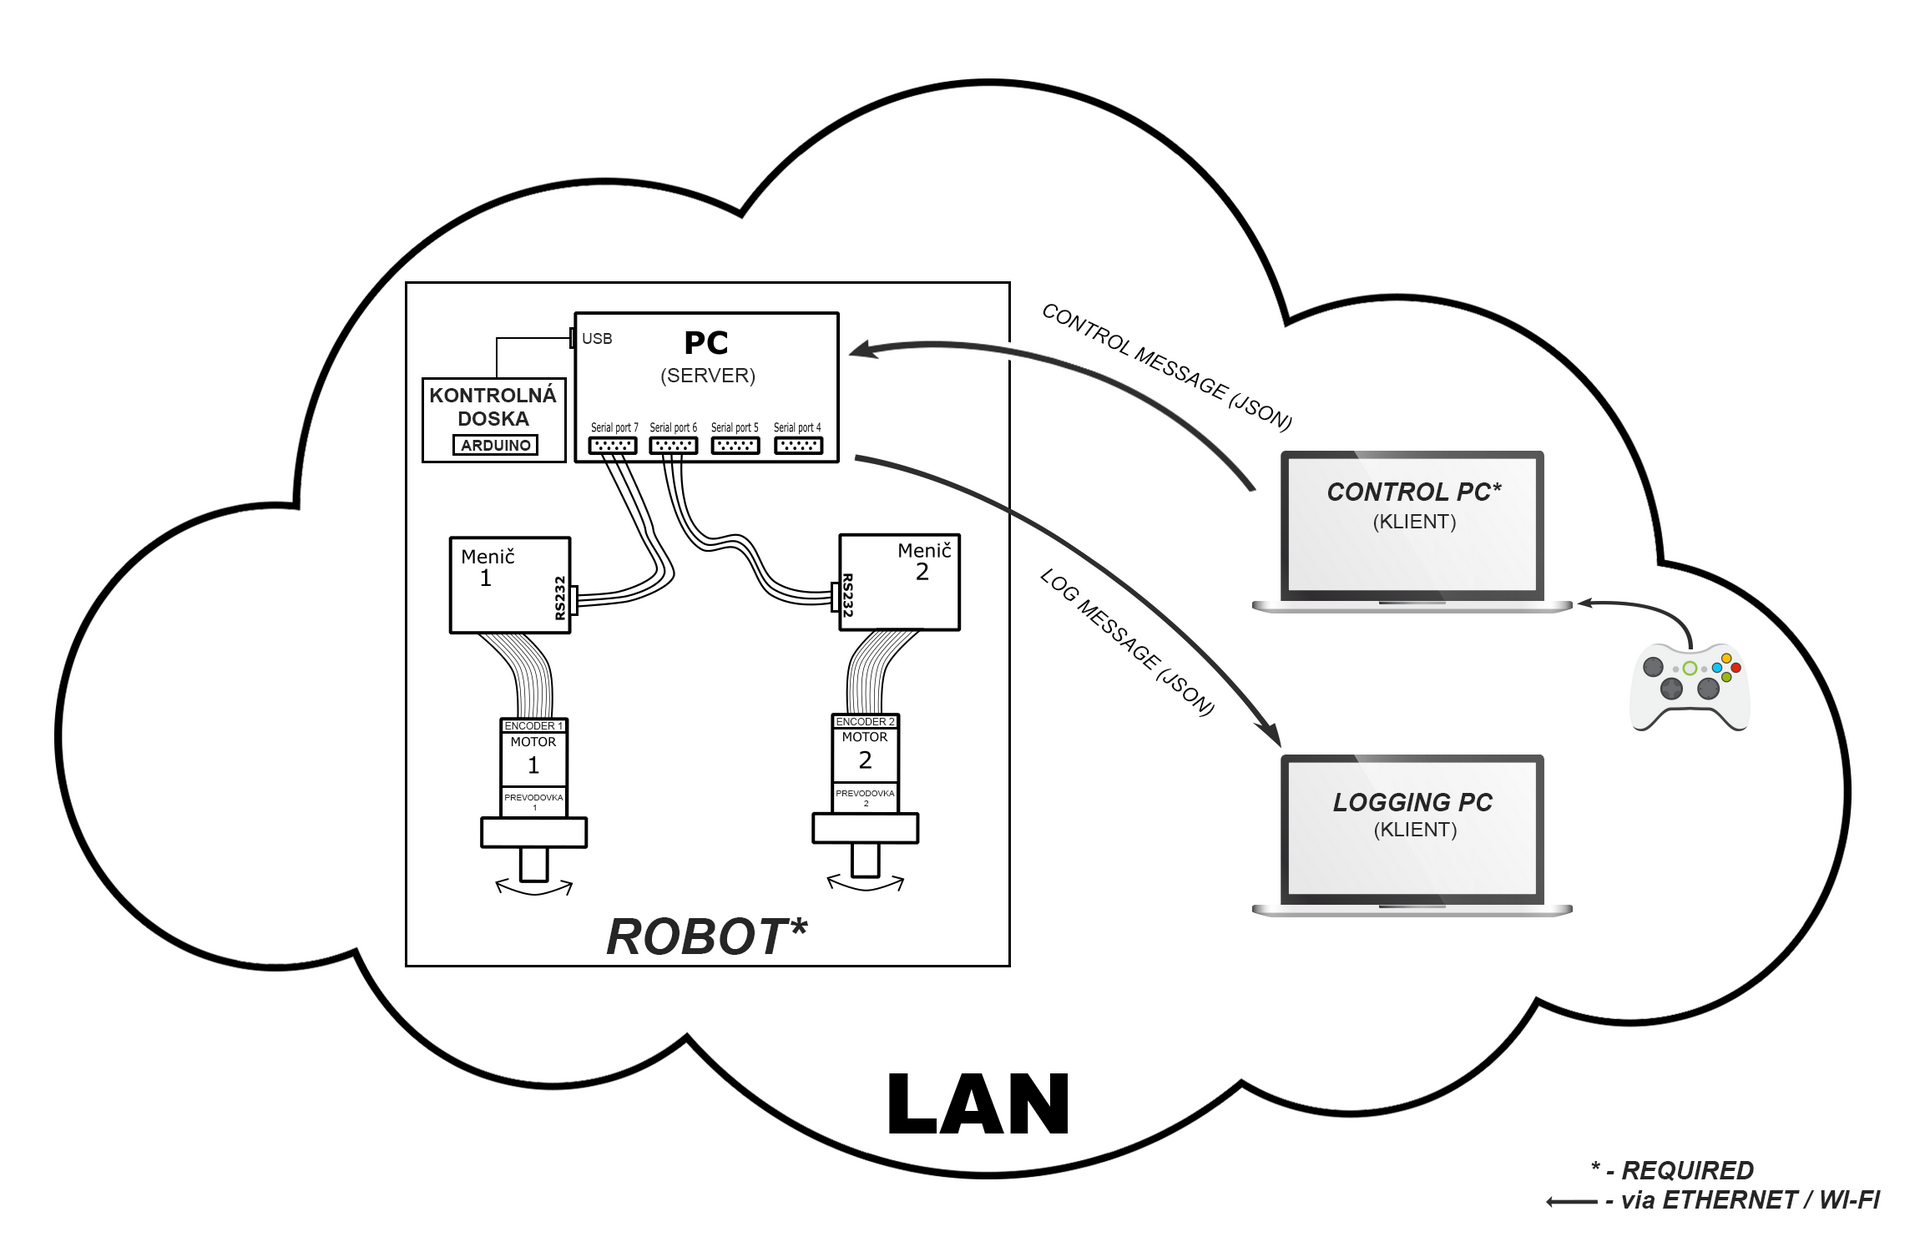
\includegraphics[width=9cm]{img/schemaRobota.png}
	\end{center}
	\caption{Schéma zapojenia jednotlivých častí na~robote}
	\label{fig:schemaRobota}
\end{figure}

Na~obrázku Obr.~\ref{fig:schemaRobota} vidíme zapojenie jednotlivých častí robota. Čo sme nespomenuli a~nachádza
sa na~obrázku je XBox ovládač je to~kvôli tomu, že~tímový projekt bol zameraný na~ovládanie robota pomocou tohto
ovládača na~počítači s~operačným systémom Windows. My tento ovládač použivať nebudeme.

\subsection{Komunikácia s~robotom}
\label{subsec:komunikacia}

S~robotom sa vieme spojiť pomocou dvoch portov. Jeden port je otvorený na~prijímanie požiadavok (requestov) a~ten
druhý je na~monitorovanie stavu robota. Port \textit{664} je otvorený pre~jedného užívateľ, ktorý môže len sledovať
stav robota. Druhý port je na~prijímanie požiadavok \textit{665} a~je taktiež otvorený len pre~jedného užívateľa.

\subsubsection{Logovanie}
\label{sec:logovanie}

	Spomínaný port \textit{664} je otvorený jednému užívateľovi. Keď sa užívateľ pripojí začne dostávať nepretržite
	správy typu \textit{JSON}~(\acrlong{JSON}), ktoré hlásia stav robota. Správy, ktoré dostávame sú~nasledujúceho
	formátu

	\begin{lstlisting}
			{"state":1,"direction":1}
	\end{lstlisting}

	Hodnoty sa pri~stave (state) a~ani pri~smere (direction) nemenia. Sú~to~stále jednotky. Pokým robot nezastavíme
	buď príkazom, alebo stlačením tlačidla vypnutia, alebo zablokovaním jedného z~kolies, tak~sa tieto správy budú
	posielať. Ak~nejaká z~týchto udalostí nastane, server prestane posielať tieto správy.

	Môžeme potom začať polemizovať o~tom či~by nebolo lepšie už~tieto správy využiť na~to~čo reálne
	spomenutý \textit{JSON} reťazec ukazuje. A~to~udávať smer a~stav robota. Momentálne tieto správy slučia len na~to,
	aby sme vedeli, že~tento robot je aktívny a~vie primať a~spracúvať informácie.

\subsubsection{Ovládanie}
\label{sec:ovladanie}

	Port \textit{665} je sprístupnený na~prijímanie a~odosielanie požiadavok a~ich odpovedí. Príkazy sa na~počítač posielajú cez~sieť z~externého
	počítača vo~formáte \textbf{JSON}. Podľa dokumentácie~\cite{BMdoc} sa robot mal ovládať správami nasledujúceho typu:

	\label{jsonSpeedRequestBad}
	\begin{lstlisting}
			{"UserID":1,"Command":3,"RightWheelSpeed":50,"LeftWheelSpeed":50}
	\end{lstlisting}

	\noindent Význam jednotlivých parametrov:
	\begin{itemize}
		\item \textbf{UserID} -- Znázorňuje ID užívateľa, ktorý je pripojený na~robot. Predvolená hodnota je 1.
		\item \textbf{Command} --  Číselná hodnota znázorňujúca príkaz, ktorý ma robot vykonať
			\begin{enumerate}
				\setcounter{enumi}{-1}
				\item \label{c0} Prázdny príkaz slúžiaci na~overenie spojenia
				\item \label{c1} Núdzové zastavenie
				\item \label{c2} Normálne zastavenie
				\item \label{c3} Príkaz nastavujúc rýchlosti kolies mobilného robota
				\item \label{c4} Prázdny príkaz
				\item \label{c5} Prázdny príkaz
				\item \label{c6} Príkaz pýtajúci si aktuálne rýchlosti pravého a~ľavého kolesa.
				\item \label{c7} Pripravenie motorov robota
				\item \label{c8} Príkaz pýtajúci si aktuálnu pozíciu pravého a~ľavého kolesa.
			\end{enumerate}
		\item \textbf{RightWheelSpeed} -- Nastavenie rýchlosti pre~pravé koleso
		\item \textbf{LeftWheelSpeed} -- Nastavenie rýchlosti pre~ľavé koleso
	\end{itemize}

	Spracovanie týchto správ je spravená v~samostatnom vlákne. Toto vlákno je vytvorené pomocou metódy \textbf{polling}.
	Neustále dookola sa volá funkcia \textit{read} (čítaj). Táto funkcia je nastavená tak, aby nezablokovala vlastné vlákno.
	Keď sa funkcia read vykonala, nezáleží na~tom či~skončila úspešne alebo nie, uspí sa vlákno prijímania správ na~100 milisekúnd.

	Študenti, ktorí navrhovali systém posielania požiadavok (request) a~odpovedí (response) robili tieto správy
	ručne. Preto~nastávajú situácie, kedy robot pošle správu, ktorá nezodpovedá štandardu písania textu v~JSON
	štandarde. Z~tohto dôvodu sme nemohli použiť už~existujúci kód na~analyzu tohto typu textu (parser), ktorý
	by nám zjednodušil prehľadávanie týchto správ.

\subsection{Vysvetlenie kľúčov reťazca}

\noindent \textbf{UserID} \newline
\indent Táto možnosť je v~momentálnom stave robota nevyužitá. Počet zariadení, ktoré sa môžu pripojiť na~port,
cez~ktorý sa dá robot ovládať je 1. Je to~ale~dobrá možnosť na~rozšírenie kódu. Keď sa budú môcť pripojiť
viacerí užívatelia, tak~sa bude musieť vyriešiť, koho príkaz bude mať akú prioritu. \newline

\noindent \textbf{Command} \newline
\indent Hodnota tohto kľúča určuje, aký príkaz sa pošle robotu na~vykonanie. Dva príkazy nie sú~implementované,
a~teda robot má možnosť na~rozšírenie svojej funkcionality. \newline

\noindent \textbf{RightWheelSpeed/LeftWheelSpeed} \newline
\indent Nastavovanie rýchlostí pravého a~ľavého kolesa nie je povinné pri väčšine príkazov. Musíme ich zadávať
len v~prípade posielania rýchlostí cez~príkaz s~číslom \ref{c3}.
